% Template for PLoS
% Version 3.5 March 2018
%
% % % % % % % % % % % % % % % % % % % % % %
%
% -- IMPORTANT NOTE
%
% This template contains comments intended
% to minimize problems and delays during our production
% process. Please follow the template instructions
% whenever possible.
%
% % % % % % % % % % % % % % % % % % % % % % %
%
% Once your paper is accepted for publication,
% PLEASE REMOVE ALL TRACKED CHANGES in this file
% and leave only the final text of your manuscript.
% PLOS recommends the use of latexdiff to track changes during review, as this will help to maintain a clean tex file.
% Visit https://www.ctan.org/pkg/latexdiff?lang=en for info or contact us at latex@plos.org.
%
%
% There are no restrictions on package use within the LaTeX files except that
% no packages listed in the template may be deleted.
%
% Please do not include colors or graphics in the text.
%
% The manuscript LaTeX source should be contained within a single file (do not use \input, \externaldocument, or similar commands).
%
% % % % % % % % % % % % % % % % % % % % % % %
%
% -- FIGURES AND TABLES
%
% Please include tables/figure captions directly after the paragraph where they are first cited in the text.
%
% DO NOT INCLUDE GRAPHICS IN YOUR MANUSCRIPT
% - Figures should be uploaded separately from your manuscript file.
% - Figures generated using LaTeX should be extracted and removed from the PDF before submission.
% - Figures containing multiple panels/subfigures must be combined into one image file before submission.
% For figure citations, please use "Fig" instead of "Figure".
% See http://journals.plos.org/plosone/s/figures for PLOS figure guidelines.
%
% Tables should be cell-based and may not contain:
% - spacing/line breaks within cells to alter layout or alignment
% - do not nest tabular environments (no tabular environments within tabular environments)
% - no graphics or colored text (cell background color/shading OK)
% See http://journals.plos.org/plosone/s/tables for table guidelines.
%
% For tables that exceed the width of the text column, use the adjustwidth environment as illustrated in the example table in text below.
%
% % % % % % % % % % % % % % % % % % % % % % % %
%
% -- EQUATIONS, MATH SYMBOLS, SUBSCRIPTS, AND SUPERSCRIPTS
%
% IMPORTANT
% Below are a few tips to help format your equations and other special characters according to our specifications. For more tips to help reduce the possibility of formatting errors during conversion, please see our LaTeX guidelines at http://journals.plos.org/plosone/s/latex
%
% For inline equations, please be sure to include all portions of an equation in the math environment.
%
% Do not include text that is not math in the math environment.
%
% Please add line breaks to long display equations when possible in order to fit size of the column.
%
% For inline equations, please do not include punctuation (commas, etc) within the math environment unless this is part of the equation.
%
% When adding superscript or subscripts outside of brackets/braces, please group using {}.
%
% Do not use \cal for caligraphic font.  Instead, use \mathcal{}
%
% % % % % % % % % % % % % % % % % % % % % % % %
%
% Please contact latex@plos.org with any questions.
%
% % % % % % % % % % % % % % % % % % % % % % % %

\documentclass[10pt,letterpaper]{article}
\usepackage[top=0.85in,left=2.75in,footskip=0.75in]{geometry}

% amsmath and amssymb packages, useful for mathematical formulas and symbols
\usepackage{amsmath,amssymb}

% Use adjustwidth environment to exceed column width (see example table in text)
\usepackage{changepage}

% Use Unicode characters when possible
\usepackage[utf8x]{inputenc}

% textcomp package and marvosym package for additional characters
\usepackage{textcomp,marvosym}

% cite package, to clean up citations in the main text. Do not remove.
% \usepackage{cite}

% Use nameref to cite supporting information files (see Supporting Information section for more info)
\usepackage{nameref,hyperref}

% line numbers
\usepackage[right]{lineno}

% ligatures disabled
\usepackage{microtype}
\DisableLigatures[f]{encoding = *, family = * }

% color can be used to apply background shading to table cells only
\usepackage[table]{xcolor}

% array package and thick rules for tables
\usepackage{array}

% create "+" rule type for thick vertical lines
\newcolumntype{+}{!{\vrule width 2pt}}

% create \thickcline for thick horizontal lines of variable length
\newlength\savedwidth
\newcommand\thickcline[1]{%
  \noalign{\global\savedwidth\arrayrulewidth\global\arrayrulewidth 2pt}%
  \cline{#1}%
  \noalign{\vskip\arrayrulewidth}%
  \noalign{\global\arrayrulewidth\savedwidth}%
}

% \thickhline command for thick horizontal lines that span the table
\newcommand\thickhline{\noalign{\global\savedwidth\arrayrulewidth\global\arrayrulewidth 2pt}%
\hline
\noalign{\global\arrayrulewidth\savedwidth}}


% Remove comment for double spacing
%\usepackage{setspace}
%\doublespacing

% Text layout
\raggedright
\setlength{\parindent}{0.5cm}
\textwidth 5.25in
\textheight 8.75in

% Bold the 'Figure #' in the caption and separate it from the title/caption with a period
% Captions will be left justified
\usepackage[aboveskip=1pt,labelfont=bf,labelsep=period,justification=raggedright,singlelinecheck=off]{caption}
\renewcommand{\figurename}{Fig}

% Use the PLoS provided BiBTeX style
% \bibliographystyle{plos2015}

% Remove brackets from numbering in List of References
\makeatletter
\renewcommand{\@biblabel}[1]{\quad#1.}
\makeatother



% Header and Footer with logo
\usepackage{lastpage,fancyhdr,graphicx}
\usepackage{epstopdf}
%\pagestyle{myheadings}
\pagestyle{fancy}
\fancyhf{}
%\setlength{\headheight}{27.023pt}
%\lhead{
\includegraphics[width=2.0in]{PLOS-submission.eps}}
\rfoot{\thepage/\pageref{LastPage}}
\renewcommand{\headrulewidth}{0pt}
\renewcommand{\footrule}{\hrule height 2pt \vspace{2mm}}
\fancyheadoffset[L]{2.25in}
\fancyfootoffset[L]{2.25in}
\lfoot{\today}

%% Include all macros below

\newcommand{\lorem}{{\bf LOREM}}
\newcommand{\ipsum}{{\bf IPSUM}}


% Pandoc citation processing
\newlength{\csllabelwidth}
\setlength{\csllabelwidth}{3em}
\newlength{\cslhangindent}
\setlength{\cslhangindent}{1.5em}
% for Pandoc 2.8 to 2.10.1
\newenvironment{cslreferences}%
  {}%
  {\par}
% For Pandoc 2.11+
\newenvironment{CSLReferences}[2] % #1 hanging-ident, #2 entry spacing
 {% don't indent paragraphs
  \setlength{\parindent}{0pt}
  % turn on hanging indent if param 1 is 1
  \ifodd #1 \everypar{\setlength{\hangindent}{\cslhangindent}}\ignorespaces\fi
  % set entry spacing
  \ifnum #2 > 0
  \setlength{\parskip}{#2\baselineskip}
  \fi
 }%
 {}
\usepackage{calc} % for calculating minipage widths
\newcommand{\CSLBlock}[1]{#1\hfill\break}
\newcommand{\CSLLeftMargin}[1]{\parbox[t]{\csllabelwidth}{#1}}
\newcommand{\CSLRightInline}[1]{\parbox[t]{\linewidth - \csllabelwidth}{#1}\break}
\newcommand{\CSLIndent}[1]{\hspace{\cslhangindent}#1}




\usepackage{forarray}
\usepackage{xstring}
\newcommand{\getIndex}[2]{
  \ForEach{,}{\IfEq{#1}{\thislevelitem}{\number\thislevelcount\ExitForEach}{}}{#2}
}

\setcounter{secnumdepth}{0}

\newcommand{\getAff}[1]{
  \getIndex{#1}{Universitat de Barcelona (UB),Vall d'Hebron Research
Institute (VHIR)}
}

\providecommand{\tightlist}{%
  \setlength{\itemsep}{0pt}\setlength{\parskip}{0pt}}

\begin{document}
\vspace*{0.2in}

% Title must be 250 characters or less.
\begin{flushleft}
{\Large
\textbf\newline{\emph{A heuristic algorithm to select genes potentially
regulated by
methylation}} % Please use "sentence case" for title and headings (capitalize only the first word in a title (or heading), the first word in a subtitle (or subheading), and any proper nouns).
}
\newline
% Insert author names, affiliations and corresponding author email (do not include titles, positions, or degrees).
\\
Alex Sanchez-Pla\textsuperscript{\getAff{Universitat de Barcelona
(UB)}, \getAff{Vall d'Hebron Research Institute
(VHIR)}}\textsuperscript{*},
Berta Miro\textsuperscript{\getAff{Vall d'Hebron Research Institute
(VHIR)}}\\
\bigskip
\textbf{\getAff{Universitat de Barcelona (UB)}}Departament of Genetics
Microbiology and Statistics, Avda Diagonal 645, Barcelona, 08028\\
\textbf{\getAff{Vall d'Hebron Research Institute (VHIR)}}Statistics and
Bioinformatics Unit (UEB), Passeig de la Vall d'Hebron 119-129,
Barcelona, 08035\\
\bigskip
* Corresponding author: asanchez@ub.edu\\
\end{flushleft}
% Please keep the abstract below 300 words
\section*{Abstract}
Methylation is key process in cancer. It usually acts by inhibiting the
expression of the gene. However, when methylation is low, any values of
gene expression can be found for that given gene. This suggests that, to
select genes regulated by methylation, one may look for patterns in the
relationship between gene expression and methylation that show either an
``L-shape'' or a negative correlation between expression and
methylation. To that end, we have developed a heuristic algorithm that
mimics the process of visually selecting an ``L-shape,'' where genes can
show a wide range of expression values (from low to high) when
methylation is low, but only low expression for intermediate or high
methylation. The method has been implemented in an R package,
``Lheuristic'' and a Shiny application, both available from GitHub
(http://github.com/alexsanchezpla). For two given two matrices - for
expression and methylation values and with the same row and column names
- the program offers the possibility to select genes based on either
negative correlation, the heuristic algorithm or both methods at once.
Once genes have been selected, results can be interactively reviewed,
plotted or downloaded. The method shows good performance when compared
against the naïve correlation, especially due to its flexibility.

% Please keep the Author Summary between 150 and 200 words
% Use first person. PLOS ONE authors please skip this step.
% Author Summary not valid for PLOS ONE submissions.

\linenumbers

% Use "Eq" instead of "Equation" for equation citations.
\hypertarget{introduction-and-background}{%
\section{Introduction and
Background}\label{introduction-and-background}}

\hypertarget{introduction-to-methylation}{%
\subsection{Introduction to
methylation}\label{introduction-to-methylation}}

Epigenetic marks modulate gene expression without affecting the DNA
nucleotide sequence. These potentially heritable changes are, for
example, DNA methylation or histone acetylation ({[}1{]}). DNA
methylation is the most studied epigenetic process in humans. The
process is based on the addition of a methyl group, mostly in CpG
dinucleotides. The CpG dinucleotides tend to group in areas of less than
500kb and with higher than 55\% C and G content , these regions are
named islands; further from the island the region is called shore and
further from the shore it is called shelf. More than 60\% of promoter
regions are associated with CpG islands ({[}2{]}) and the methylation of
these is linked to gene silencing and gene expression inhibition. DNA
methylation has been linked to the regulation of numerous cellular
processes, including embryonic development, or X-chromosome inactivation
and preservation of chromosome stability among others. DNA methylation
has also been observed in autoimmune diseases, metabolic disorders,
neurological disorders, and other processes that despite being natural
they are debilitating, like ageing for example; and it can also be
correlated with drug or treatment response ({[}3{]}; {[}4{]}; {[}5{]};
{[}6{]}). Most research on this area has been, however, focused on tumor
repressor genes, which are often silenced in cancer cells due to
hypermethylation. This is an important mechanism of gene silencing
during tumor progression ({[}7{]}). On the contrary, a general level of
hypomethylation has been observed in human tumors ({[}8{]}); therefore,
hypomethylation is a useful mechanism to distinguish genes of some human
cancers from their normal counterparts.\\
In the human genome, about 80\% of cytosines in the 56 million CpG sites
are methylated to 5-methylcytosines. The methylation pattern of DNA is
highly variable among cells types and developmental stages and
influenced by disease processes and genetic factors. The relationship
between gene expression and methylation has been associated with cancer
and extensively studied, therefore it has produced fruitful results
({[}9{]}).

\hypertarget{analysis-of-genes-regulatated-by-methylation}{%
\subsection{Analysis of genes regulatated by
methylation}\label{analysis-of-genes-regulatated-by-methylation}}

With the abundance of emerging evidence indicating the important role of
DNA methylation in common diseases, researchers have attempted to use
DNA methylation as a biomarker to identify epigenetic changes that are
associated with disease status. While the genetic events that drive the
tumorigenic process are relatively well characterized for colorectal
cancer, the epigenetic events and their impact on the transcriptional
reprogramming observed in colorectal tumors have not been extensively
characterized. Although recent genome-wide studies have analyzed the
genomic distribution of hypermethylated CpGs in a small number of
colorectal tumors ({[}10{]}; {[}11{]}; {[}12{]}), a detailed analysis of
the subset of these events that are important for gene expression
regulation is currently lacking. Just as gene expression microarrays
accelerated and revolutionized the study of transcriptional regulation,
rapidly improving technologies are increasingly enabling researchers to
assess locus-specific DNA methylation on a genome-wide scale. Recently
various high-throughput approaches based on bisulfite conversion
combined with next generation sequencing have been developed and applied
for the genome wide analysis of DNA methylation. These methods provide
single base pair resolution, quantitative DNA methylation data with
genome wide coverage. There are various experimental types of
methylation assays, but overall, methylation levels can be represented
in one of three types: discrete, continuous or categorical. Therefore,
methylation can be quantified by directly using read count information ,
ratio data (which may lose biological variability) or both. Once the DNA
samples are processed, an important issue to be considered is the
influence of the statistical analysis on the accuracy of the genomic
methylation level estimation from bisulfite sequencing data. The
accuracy of the statistical approach to methylation quantification
increases with the sequencing depth of the particular cytosine residue
({[}13{]}). However, there are regression and neighboring analysis
techniques that can counteract the lack of sequence depth in a
particular CpG ({[}14{]}).

\hypertarget{existing-methods-and-analyses}{%
\subsubsection{Existing methods and
analyses}\label{existing-methods-and-analyses}}

The association between gene expression and DNA methylation in the CpG
islands in particular has been long studied; and as a result, mostly
negative correlations have been found to relate to cancer driven
mechanisms ({[}15{]}), but this inverse relationship between DNA
methylation of the first intron in particular and gene expression is a
broad mechanism to down-regulate gene expression and it is found in
numerous processes, organisms and tissues ({[}16{]}). There have been
various studies analysing this correlation using various approaches. For
example, Massie et al., (2017) looked at the relationship between gene
expression and DNA methylation at the probe level rather than at the
gene level. They narrowed a list of genes regulated by methylation that
were identified in more than 3 out of 17 studies ({[}17{]}). Another
study analysed the TCGA database to identify patterns in DNA CpG
methylation and gene expression and tumor status. They found that the
association involved a reduced number of genes linked to cancer than
originally anticipated (around the hundreds) and that not all
correlations were negative ({[}18{]}). Another recent paper reported two
different models for analysis of DNA methylation and regulation of gene
expression, one for negatively correlated genes and one for positively
correlated genes ({[}19{]}). They used expression (GSE106582) and
methylation datasets (GSE101764) containing 194 samples, 77 tumors and
117 of the mucose. By random forest analysis they were able to classify
genes into cancer related and not related. Still methodologies to find
tune classification into cancer/disease related and not cancer/disease
related are still needed. A previously developed method was the
selection of genes with an L-shape association between the expression
and the methylation datasets ({[}20{]}). In this research, they focused
on the CMI and on a method based on spline regression. They observed
that the first method would detect L-shaped genes more accurately in big
datasets. On the other hand, the splines clustering was not size
dependent, but it would yield a smaller number of samples. Other
research exists that aimed to identify genes regulated by methylation
according to the expression methylation patterns; however, they only use
a particular methodology like the CMI ({[}21{]}) with positive results.
A paper focused on the identification of genes regulated by methylation
through unsupervised clustering techniques to identify CRC subtypes was
able to confirm existing subtypes ({[}22{]}).There has been other work
that focused on the development of platforms for the identification of
genes regulated by methylation. One of these packages is MEXPRESS
({[}\textbf{Koch2015?}{]}). This package has a web interface that allows
the user to visualize expression and methylation data from genes in the
TCGA data. The visualization collocates for each selected gene, CpG
islands, with transcripts expression together with other clinical values
such as gender and age. The tool also generates p-values in relation to
the variables specified. Another one of these packages is Methylmix
({[}\textbf{Gevaert2015?}{]}). The algorithm is based on a beta mixture
model that identifies methylation states and compares them with what
they call normal conditions to find hypo- and hyper-methylated genes.
They developed a new statistic coeficient, the Differential Methylation
value or DM-value which is defined as the difference of a methylation
state with the normal methylation state. Then, they correlate that
coefficient with gene expression data to characterize the association
between methylation level and gene expression. For expression and
methylation correlation analyses of both RNA and DNA molecules there is
also a web based tool that analyses methylated genes based on TCGA data,
called MethHC (http://methhc.mbc.nctu.edu.tw/php/search.php?opt=gene,
{[}\textbf{Huang2015?}{]}). This database has an analysis tool that
provides gene-specific analysis for various diseases, and the
information is displayed as a comparison between diseased and normal
(non-diseased) conditions; list of highest and lowest methylated (hyper
and hypo) genes; as well as correlations between expression and
methylation. In this, methylation is a binary value (0,1). Other
methodologies to identify methylated genes associated with cancer is
through text mining analysis, as in the PubMeth database
(www.pubmeth.org, {[}23{]}). In this, they identified 5000 genes of 1000
publications. However, high-throughput methodologies that offer an
impartial approach to the identification of genes regulated by
methylation still need further development and fine-tuning. Here we
present such a methodology that will select, out of a gene expression
and DNA methylation subsets, those genes that present a negative
correlation, and are therefore regulated by methylation. The L-shaped
heuristic method to identify genes regulated by methylation was tested
and tuned for experimental expression and methylation paired datasets
after normalization using other standard methods.

\hypertarget{materials-and-methods}{%
\section{Materials and Methods}\label{materials-and-methods}}

As we have described in the previous section, although there are various
approaches to selecting genes based on the relationship between
methylation levels and gene expression, none of them are completely
satisfactory.

In this section we present the method we have developed to select genes
in which the pattern of the relationship is ``L-shaped.'' In fact,
taking biological processes into account, this is a very common and very
reasonably expected pattern when genes are regulated by methylation.
Furthermore, as we will see later, it is not only important but can be
partially missed by ``naïve'' methods such as significant negative
correlation, which increases the interest of our proposal.

\hypertarget{rationale-of-the-approach}{%
\subsection{Rationale of the approach}\label{rationale-of-the-approach}}

After trying different approaches to detect L-shapes, one often comes
back to an intuïtive idea: If we are looking for genes whose expression
can take any value when methylation is low, and tends to decrease as
methylation increases one should observe that points in the
methylation-expression scatterplot tend to be scattered near the
vertical and horizontal positive axes showing an L-shape. If this does
not happen genes can be found anywhere in the scatterplot and we can
call it a non-L-shape. That is:

\begin{itemize}
\tightlist
\item
  The more the points cluster near the vertical and horizontal axes, the
  more L-shaped can be considered the scatterplot.
\item
  The more the points move away from the axes, the least L-shaped the
  scatterplot is.
\end{itemize}

This representation of differing scatterplot patterns can be observed in
two real but non-identified genes from a colorectal cancer study (Fig.
1).

\hypertarget{an-algorithm-to-select-l-shape-scatterplots}{%
\subsection{An algorithm to select L-shape
scatterplots}\label{an-algorithm-to-select-l-shape-scatterplots}}

Assuming that genes potentially regulated by methylation can be selected
from between L-shaped expression--methylation scatterplots, finding a
way to separate L-shape from non-L shape ones is a reasonable first
step. It could be argued that this could be done manually, but given the
high number of -possibly highly variable- figures to be searched, an
algorithm to automate this process is a much better option.

The algorithm can be developed starting from the intuitive distinction
between L and non-L discussed above and making it more explicit as
follows:

\begin{enumerate}
\item Given a scatterplot methylation-expression $X$, overlay a $k\times m$ grid on it so that each point is assigned to one and only one of the grid's cell. Usually $k=m=3$ so this will be the values used in the following.
\item Classify the scatterplot as \textbf{``L'' or ``non-L''} based on a small set of conditions:
\begin{enumerate}
  \item There must be a \emph{minimum} number of points in the upper-left (cell (1,1)) and lower right (cell (3,3)) corners of the grid.
  \item There must be a \emph{maximum} number of points in the upper right (cell (1,3)) because points there mean hypermethylation and hyperexpression which is the opposite of what we are looking for.
  \item We will usually \emph{not require to have a minimum of points in cell (3,1)} unless we are really willing to have an L-shape (in our setting we will also be happy tho recover diagonals, which also reflect a negative correlation!).
\end{enumerate}
\item Score points on each subgrid in such a way that
\begin{enumerate}
    \item Points in permitted regions (left-outer margin, i.e. cells: (1,1), (2,2), (3,1), (3,2), (3,3)) score positively if the scatterplot has been classified as L or zero if it has been classified as non-L.
    \item Points in non-desired regions (outer band. i.e. cells (1,2), (1,3), (2,3)) score negatively in all cases.
    \item Some regions may be declared neutral and not-score, such as cell (2,2).
\end{enumerate}
\item Use cross-validation to tune scoring parameters (\textit{if a set of positive and negative L-shaped genes is available}). 
\end{enumerate}

The previous scheme can be summarized using the following equation.
\begin{equation}
S(X) = W_L \circ X \times \mathbf{1}_L(X) + W_{L^C} \circ X \times \mathbf{1}_{L^c}(X),
\end{equation} where

\begin{itemize}
\item ${X}$ is the matrix of \emph{counts}, i.e. the number of counts in each cell of the grid,
\item ${W_L}$ is the matrix of scores per cell and point \emph{if the scatterplot has been classified as $L$},
\item ${W_{L^c}}$ is the matrix of scores per cell and point \emph{if the scatterplot has been classified as non-$L$ ($L^c$)},
\end{itemize}

and \(\circ\) represents the hadamard product of the two matrices
\(W_{L/L^c}\) (i.e.~elementwise multiplication of the two matrices) and
\(\mathbf{1}_{L/L^c}()\) is the indicator function for \(L\) or \(L^c\).

The fact that the scatterplot is assigned to \(L\) or \(L^c\) can also
be described as the hadamard product of three matrices: \begin{equation}
\mathbf{1}_L(X) = \bigwedge_{i,j} X \circ C \circ \left( mMP \times \sum_{i,j}x_{ij}\right),
\end{equation} where

\begin{itemize}
\item ${X}$ is the matrix of \emph{counts}, i.e. the number of counts in each cell of the grid,
\item $C$ is the matrix of conditions to be verified \emph{if the scatterplot has to be classified as $L$},
\item $mMP$ is the matrix of minimum and Maximum Percentages of points to have in each cell \emph{if the scatterplot has to be classified as $L$},
\item $\circ$ represents the pointwise logical operation which allows that the product of the three cells becomes a logical operation and
\item $\bigwedge_{i,j}$ represents an logical ``AND'' operation of all cells, that is if all cells are TRUE the result is assigned to $L$ and if one fails it is assigned to $L^c$.
\end{itemize}

Fig. 2 shows a graphic representation of this grid approach.

\hypertarget{synthetic-dataset-generation-for-the-simulation-studies}{%
\subsection{Synthetic dataset generation for the simulation
studies}\label{synthetic-dataset-generation-for-the-simulation-studies}}

The R package \texttt{simstudy} was used to create 4 artificial datasets
by using the splines method
(https://cran.r-project.org/web/packages/simstudy/simstudy.pdf). The
package allows for designing data points on a pre-defined spline, in
which knots, limits and dispersion can be tuned. The splines are
generated based on a fixed X variable representing the methylation
values. The artificial datasets contained a total of 1000 genes, and the
data points were developed based on 2 parameters with 2 levels each. The
first parameter was the number of samples and the second the \% of true
regulated by methylation genes that a sample would contain (with an
expression by methylation scatterplot or spline following an L-shape).
The number of samples considered was of 50 and 1000, and the \% of true
methylated genes in each dataset was 1\% and 10\%. Additionally, the
shape of the negative genes (not regulated by methylation) was also
pre-defined and classified into 5 different scatterplot patterns (Fig.
3) and the percentage of genes in each category equaled to 1/3 prior
subtraction of the true GRM genes. These artificial genes were generated
based on real gene patterns observed from a colorectal cancer study
(Fig. 4).

\hypertarget{tuning-of-parameters}{%
\subsection{Tuning of parameters}\label{tuning-of-parameters}}

\hypertarget{results}{%
\section{Results}\label{results}}

\hypertarget{detection-of-l-and-no-l-scatterplots-with-the-heuristic-algorithm-using-the-synthetic-dataset}{%
\subsection{Detection of L and no-L scatterplots with the heuristic
algorithm using the synthetic
dataset}\label{detection-of-l-and-no-l-scatterplots-with-the-heuristic-algorithm-using-the-synthetic-dataset}}

The heuristic method was tested with the 4 artificial datasets
previously described: 50 samples, 1\% of GRM genes; 50 samples, 10\% GRM
genes; 1000 samples, 1\% GRM genes; and 1000 samples, 10\% GRM genes.
After running the model, sensitivity, specificity, and accuracy were
measured and compared between datasets.

\hypertarget{measures-of-performance-for-the-heuristic-method-with-synthetic-datasets}{%
\subsubsection{Measures of performance for the heuristic method with
synthetic
datasets}\label{measures-of-performance-for-the-heuristic-method-with-synthetic-datasets}}

Sensitivity, specificity and accuracy for the heuristic model were
measured for the 4 synthetic datasets (Fig. {[}ssa{]}) with the
predefined parameters described in the above section. Specificity was
the parameter that scored highest in all datsets, with values between
0.99 (for the datasets with 50 samples) and 1 (for the datasets with
1000 samples). The second highest parameter was accuracy. In this, both
datasets containing 1\% of GRM genes scored 0.99, whereas the datasets
with 10\% of GRM genes scored 0.93 (for the one with 50 samples) and
0.92 (for the one with 1000 samples). Finally, the sensitivity values
were the lowest in the combination of 1\% GRM and 1000 samples (0.1) and
highest for 1\% GRM and 50 samples (0.5). These results indicate that
the classification scored better non-L shaped scatterplots (true
negatives) than L-shaped scatterplots (true positives).

\hypertarget{tuning-of-parameters-to-improve-method-performance}{%
\subsection{Tuning of parameters to improve method
performance}\label{tuning-of-parameters-to-improve-method-performance}}

The selection of L-shaped genes with the heuristic method depends on a
variety of parameters. Changing the parameters affects the number of
genes that will be called ``L-shaped'' so we would want to find an
optimal set of parameters for every parameter combination thus some
performance measures such as sensitivity or specificity can be
optimized.

A limitation with this approach is that it requires a set of ``TRUE
Positives'' -genes known to have L-shape- or TRUE negatives genes known
not to have L-shape- and this is very hard to obtain from experimental
samples. A way to perform a selection between the TRUE and FALSE genes
is by visually inspecting the genes and selecting two sets that can be
described as ``clearly L'' and ``clearly non-L.'' This is however fairly
accurate, a more difficult concept to execute, with the added
subjectivity to the selection, for example in samples that no that
``clear.'' To override that, synthetic datasets were created. As they
were designed based on known TRUE and FALSE patterns we were able to
evaluate the method.

\hypertarget{detection-of-l-and-no-l-scatterplots-with-the-heuristic-algorithm-using-real-datasets-tcga-and-a-colorectal-cancer-dataset}{%
\subsection{Detection of L and no-L scatterplots with the heuristic
algorithm using real datasets: TCGA and a colorectal cancer
dataset}\label{detection-of-l-and-no-l-scatterplots-with-the-heuristic-algorithm-using-real-datasets-tcga-and-a-colorectal-cancer-dataset}}

\hypertarget{discussion}{%
\section{Discussion}\label{discussion}}

\hypertarget{supporting-information}{%
\section{Supporting information}\label{supporting-information}}

\hypertarget{references}{%
\section*{References}\label{references}}
\addcontentsline{toc}{section}{References}

\clearpage

\hypertarget{figures-and-captions}{%
\section{Figures and captions}\label{figures-and-captions}}

\begin{figure}
\hypertarget{id}{%
\centering
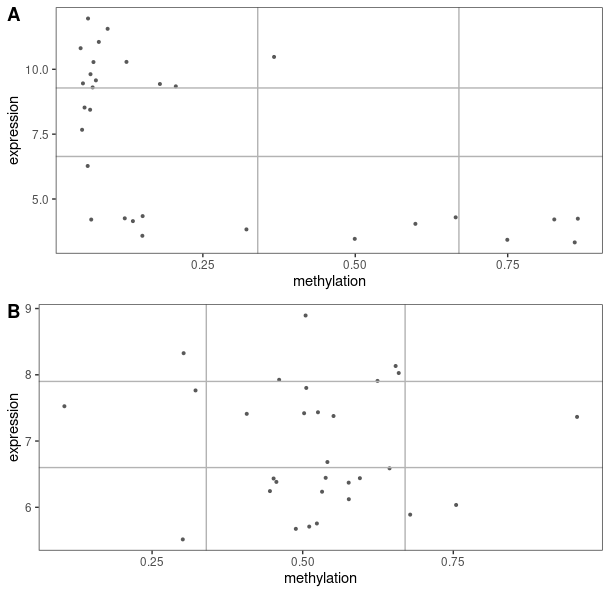
\includegraphics[width=0.5\textwidth,height=1\textheight]{figures/Figure1.png}
\caption{Example of non-Lshape vs L-shape for the
methylation--expression scatterplots associated with two real genes. A
represents a gene potentially regulated by methylation as expression
decreases with increasing methylation, giving a L--shaped scatterplot
that can be graphycally selected. B represents a gene not regulated by
methylation, since no correlation between expression and methylation
values is visible.}\label{id}
}
\end{figure}

\begin{figure}
\hypertarget{id}{%
\centering
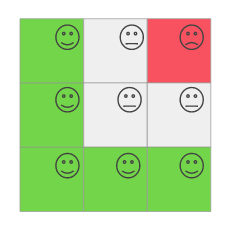
\includegraphics[width=0.5\textwidth,height=1\textheight]{figures/Figure2.png}
\caption{Grid representation to select L--shaped genes. A grid was
superimposed on the methylation--expression scatterplot graphs, each
cell representing one ninth of the graph. The grid partitioning of the
scatterplot was used to weigh the sample points so that sample points on
green cells would score higher whereas sample points on the red cell
would be penalized. Sample points distributed on the grey cells would be
given intermediatte weights}\label{id}
}
\end{figure}

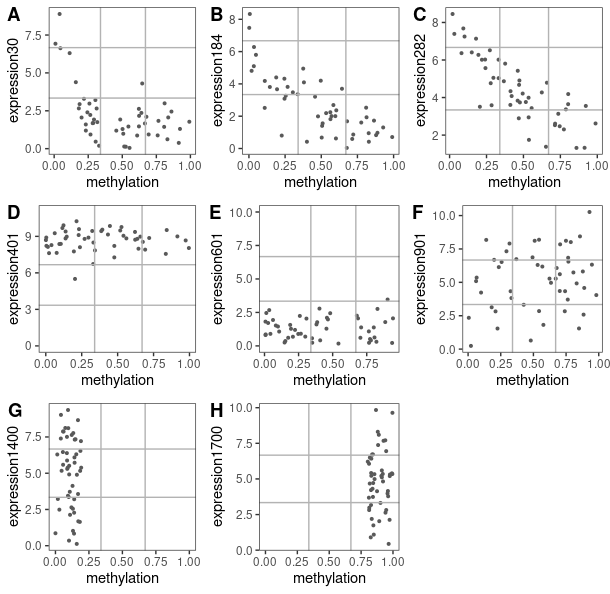
\includegraphics[width=0.5\textwidth,height=5\textheight]{figures/Figure3.png}
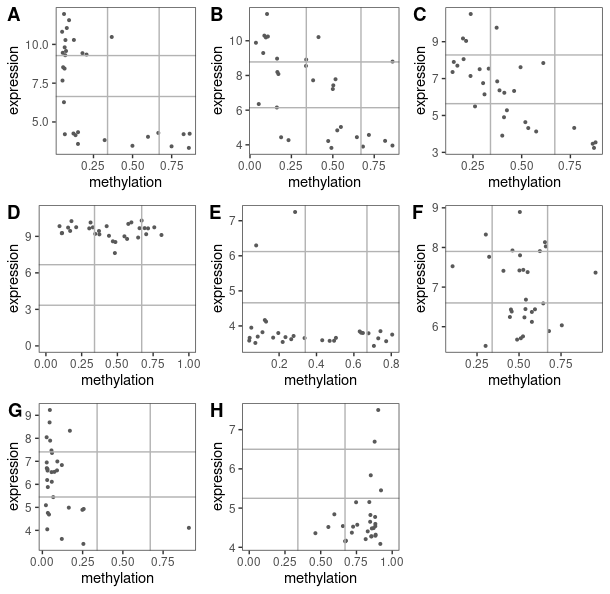
\includegraphics[width=0.5\textwidth,height=5\textheight]{figures/Figure4.png}

\hypertarget{refs}{}
\begin{CSLReferences}{0}{0}
\leavevmode\hypertarget{ref-Berger2009}{}%
\CSLLeftMargin{1. }
\CSLRightInline{Berger SL, Kouzarides T, Shiekhattar R, Shilatifard A.
{An operational definition of epigenetics}. Genes and Development.
2009;23: 781--783.
doi:\href{https://doi.org/10.1101/gad.1787609}{10.1101/gad.1787609}}

\leavevmode\hypertarget{ref-Saxonov2006}{}%
\CSLLeftMargin{2. }
\CSLRightInline{Saxonov S, Berg P, Brutlag DL. {A genome-wide analysis
of CpG dinucleotides in the human genome distinguishes two distinct
classes of promoters}. Proceedings of the National Academy of Sciences
of the United States of America. 2006;103: 1412--1417.
doi:\href{https://doi.org/10.1073/pnas.0510310103}{10.1073/pnas.0510310103}}

\leavevmode\hypertarget{ref-Reik2007}{}%
\CSLLeftMargin{3. }
\CSLRightInline{Reik W. {Stability and flexibility of epigenetic gene
regulation in mammalian development}. Nature Publishing Group; 2007. pp.
425--432.
doi:\href{https://doi.org/10.1038/nature05918}{10.1038/nature05918}}

\leavevmode\hypertarget{ref-Portela2010}{}%
\CSLLeftMargin{4. }
\CSLRightInline{Portela A, Esteller M. {Epigenetic modifications and
human disease}. 2010. pp. 1057--1068.
doi:\href{https://doi.org/10.1038/nbt.1685}{10.1038/nbt.1685}}

\leavevmode\hypertarget{ref-Feil2012}{}%
\CSLLeftMargin{5. }
\CSLRightInline{Feil R, Fraga MF. {Epigenetics and the environment:
Emerging patterns and implications}. 2012. pp. 97--109.
doi:\href{https://doi.org/10.1038/nrg3142}{10.1038/nrg3142}}

\leavevmode\hypertarget{ref-Benayoun2015}{}%
\CSLLeftMargin{6. }
\CSLRightInline{Benayoun BA, Pollina EA, Brunet A. {Epigenetic
regulation of ageing: Linking environmental inputs to genomic
stability}. Nature Publishing Group; 2015. pp. 593--610.
doi:\href{https://doi.org/10.1038/nrm4048}{10.1038/nrm4048}}

\leavevmode\hypertarget{ref-Jones2002}{}%
\CSLLeftMargin{7. }
\CSLRightInline{Jones PA, Baylin SB. {The fundamental role of epigenetic
events in cancer}. 2002. pp. 415--428.
doi:\href{https://doi.org/10.1038/nrg816}{10.1038/nrg816}}

\leavevmode\hypertarget{ref-Feinberg1983}{}%
\CSLLeftMargin{8. }
\CSLRightInline{Feinberg AP, Vogelstein B. {Hypomethylation
distinguishes genes of some human cancers from their normal
counterparts}. Nature. 1983;301: 89--92.
doi:\href{https://doi.org/10.1038/301089a0}{10.1038/301089a0}}

\leavevmode\hypertarget{ref-Yang2014}{}%
\CSLLeftMargin{9. }
\CSLRightInline{Yang X, Han H, DeCarvalho DD, Lay FD, Jones PA, Liang G.
{Gene body methylation can alter gene expression and is a therapeutic
target in cancer}. Cancer Cell. Cell Press; 2014;26: 577--590.
doi:\href{https://doi.org/10.1016/j.ccr.2014.07.028}{10.1016/j.ccr.2014.07.028}}

\leavevmode\hypertarget{ref-McInnes2017}{}%
\CSLLeftMargin{10. }
\CSLRightInline{McInnes Tyler, Zou Donghui, Rao Dasari S., Munro
Francesca M., Phillips Vicky L., McCall John L., et al. {Genome-wide
methylation analysis identifies a core set of hypermethylated genes in
CIMP-H colorectal cancer}. BMC Cancer. 2017;17: 228.
doi:\href{https://doi.org/10.1186/s12885-017-3226-4}{10.1186/s12885-017-3226-4}}

\leavevmode\hypertarget{ref-Dong2019}{}%
\CSLLeftMargin{11. }
\CSLRightInline{Dong Lixin, Ma Li, Ma Gloria H., Ren H. {Genome-wide
Analysis Reveals DNA Methylation Alterations in Obesity Associated with
High Risk of Colorectal Cancer}. Scientific Reports. 2019;9: 5100.
doi:\href{https://doi.org/10.1038/s41598-019-41616-0}{10.1038/s41598-019-41616-0}}

\leavevmode\hypertarget{ref-Orjuela2020}{}%
\CSLLeftMargin{12. }
\CSLRightInline{Orjuela Stephany, Menigatti Mirco, Schraml Peter,
Kambakamba Patryk, Robinson Mark D., Marra G. {The DNA hypermethylation
phenotype of colorectal cancer liver metastases resembles that of the
primary colorectal cancers}. BMC Cancer. 2020;20: 290.
doi:\href{https://doi.org/10.1186/s12885-020-06777-6}{10.1186/s12885-020-06777-6}}

\leavevmode\hypertarget{ref-Zhang2010}{}%
\CSLLeftMargin{13. }
\CSLRightInline{Zhang Y, Jeltsch A. {The application of next generation
sequencing in DNA methylation analysis}. 2010. pp. 85--101.
doi:\href{https://doi.org/10.3390/genes1010085}{10.3390/genes1010085}}

\leavevmode\hypertarget{ref-Wreczycka2017}{}%
\CSLLeftMargin{14. }
\CSLRightInline{Wreczycka K, Gosdschan A, Yusuf D, Grüning B, Assenov Y,
Akalin A. {Strategies for analyzing bisulfite sequencing data}. Journal
of Biotechnology. 2017;261: 105--115.
doi:\href{https://doi.org/10.1016/j.jbiotec.2017.08.007}{10.1016/j.jbiotec.2017.08.007}}

\leavevmode\hypertarget{ref-Sadikovic2008}{}%
\CSLLeftMargin{15. }
\CSLRightInline{Sadikovic B, Al-Romaih K, Squire J A, Zielenska M. Cause
and consequences of genetic and epigenetic alterations in human cancer.
Current Genomics. 2008;9: 394--408.
doi:\href{https://doi.org/10.2174/138920208785699580}{10.2174/138920208785699580}}

\leavevmode\hypertarget{ref-Anastasiadi2018}{}%
\CSLLeftMargin{16. }
\CSLRightInline{Anastasiadi D, Esteve-Codina A, Piferrer F. {Consistent
inverse correlation between DNA methylation of the first intron and gene
expression across tissues and species}. Epigenetics and Chromatin.
BioMed Central Ltd.; 2018;11.
doi:\href{https://doi.org/10.1186/s13072-018-0205-1}{10.1186/s13072-018-0205-1}}

\leavevmode\hypertarget{ref-Massie2017}{}%
\CSLLeftMargin{17. }
\CSLRightInline{Massie CE, Mills IG, Lynch AG. The importance of DNA
methylation in prostate cancer development. The Journal of Steroid
Biochemistry and Molecular Biology. 2017;166: 1--15.
doi:\url{https://doi.org/10.1016/j.jsbmb.2016.04.009}}

\leavevmode\hypertarget{ref-Long2017}{}%
\CSLLeftMargin{18. }
\CSLRightInline{Long MD, Smiraglia DJ, Campbell MJ. {The Genomic Impact
of DNA CpG Methylation on Gene Expression; Relationships in Prostate
Cancer.} Biomolecules. Multidisciplinary Digital Publishing Institute
(MDPI); 2017;7.
doi:\href{https://doi.org/10.3390/biom7010015}{10.3390/biom7010015}}

\leavevmode\hypertarget{ref-Klett2018}{}%
\CSLLeftMargin{19. }
\CSLRightInline{Klett Hagen, Balavarca Yesilda, Toth Reka, Gigic
Biljana, Habermann Nina, Scherer Dominique, et al. Robust prediction of
gene regulation in colorectal cancer tissues from DNA methylation
profiles. Epigenetics. 2018;13: 386--397.
doi:\href{https://doi.org/10.1080/15592294.2018.1460034}{10.1080/15592294.2018.1460034}}

\leavevmode\hypertarget{ref-Sanchez-Pla2017}{}%
\CSLLeftMargin{20. }
\CSLRightInline{Sánchez-Pla Alex, Ruíz de Villa M. Carme, Carmona
Francesc, Bazzoco Sarah, del Corro DA. Integrative analysis to select
genes regulated by methylation in a cancer colon study. Ainsbury
Elizabeth A., Calle M.Luz, Cardis Elisabeth, Einbeck Jochen, Gómez
Guadalupe, Puig P, editors. Springer International Publishing; 2017. pp.
53--57. doi:\url{https://doi.org/10.1007/978-3-319-55639-0_9}}

\leavevmode\hypertarget{ref-Liu2012}{}%
\CSLLeftMargin{21. }
\CSLRightInline{Liu Y, Qiu P. Integrative analysis of methylation and
gene expression data in TCGA. Proceedings 2012 IEEE international
workshop on genomic signal processing and statistics (GENSIPS). 2012.
pp. 1--4.
doi:\href{https://doi.org/10.1109/GENSIPS.2012.6507712}{10.1109/GENSIPS.2012.6507712}}

\leavevmode\hypertarget{ref-Barat2015}{}%
\CSLLeftMargin{22. }
\CSLRightInline{Barat A, Ruskin H, Byrne A, Prehn J. {Integrating Colon
Cancer Microarray Data: Associating Locus-Specific Methylation Groups to
Gene Expression-Based Classifications}. Microarrays. MDPI AG; 2015;4:
630--646.
doi:\href{https://doi.org/10.3390/microarrays4040630}{10.3390/microarrays4040630}}

\leavevmode\hypertarget{ref-Ongenaert2007}{}%
\CSLLeftMargin{23. }
\CSLRightInline{Ongenaert M, Van Neste L, De Meyer T, Menschaert G,
Bekaert S, Van Criekinge W. {PubMeth: a cancer methylation database
combining text-mining and expert annotation}. Nucleic Acids Research.
2007;36: D842--D846.
doi:\href{https://doi.org/10.1093/nar/gkm788}{10.1093/nar/gkm788}}

\end{CSLReferences}

\nolinenumbers


\end{document}
